\nonstopmode
\documentclass[]{beamer}
\usepackage{gyatheme}
\usepackage[MeX]{polski}
\usepackage[utf8x]{inputenc}
\usepackage{graphicx}
\usepackage{floatflt}
\usepackage{algorithmic}

\beamertemplateballitem
\beamertemplatenumberedballsectiontoc

\title[Płatki Śniegu]{Formowanie się płatków śniegu\\Symulacja agentowa}
\author{Marta Anna Ziobro, Jan Filipowski}
\date{\today}

\begin{document}

\begin{frame}
	\titlepage
\end{frame}

\section{Fizyka}


\begin{frame}
	\frametitle{Wzrost}
	\begin{block}{Główne procesy}
		Formowanie się płatka zależy głównie od równowagi pomiędzy Szlifowaniem a Rozgałęzianiem. Podczas Szlifowania tworzą się proste, 
		płaskie powierzchnie, Rozgałęzianie zaś dąży do udziwnienia płatka. 
		Współdziałanie tych dwóch procesów zależy w dużym stopniu od temperatury i wilgotności. 
	\end{block}
	\begin{figure}[h]
		\centering
		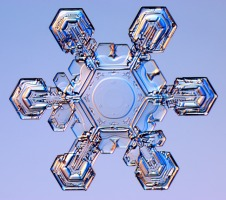
\includegraphics[width=0.9\textwidth]{crystal1.jpg}
	\end{figure}
\end{frame}


\begin{frame}
	\frametitle{Wzrost}
	\begin{figure}[h]
		\centering
		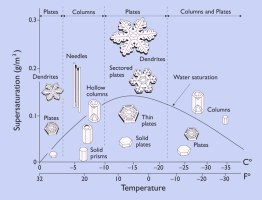
\includegraphics[width=0.9\textwidth]{morphologydiagram.jpg}
	\end{figure}
\end{frame}

\subsection{Szlifowanie kryształu}

\begin{frame}
	\frametitle{Szlifowanie}
	\begin{block}{Szlifowanie}
	Molekułom wody łatwiej przyłączać się do szorstkiej powierzchni niż gładkiej (gładka ma bowiem mniej zwisających wiązań). 
	Po tym jak wszystkie szorstkie powierzchnie się wygładzą rozpoczyna się ich powolne wzrastanie. Molekuły docelowo układają się na kracie 
	o oczku będącym sześciokątem foremnym.
	\end{block}
	\begin{figure}[h]
		\centering
		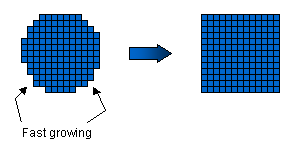
\includegraphics[width=0.4\textwidth]{facetting-square.png}
		\caption{Wygładzanie na przykładzie kwadratowej kraty}
	\end{figure}
\end{frame}


\subsection{Rozgałęzianie płatka}


\begin{frame}
	\frametitle{Rozgałęzianie}
	\begin{block}{Niestabilność rozgałęziająca}
	Molekuły wody przebywają pewną drogę w powietrzu zanim się osadzą na roznącym krysztale. 	
	Wyobrażmy sobie zatem płaską powierzchnię kryształu. Jeśli mały guz pojawi się na niej, molekułom będzie łatwiej do niego dotrzeć.
	Dlatego osadzają się na nim szybciej, a im większy się staje tym bardziej wystaje i tym szybciej rośnie. 
	\end{block}
	\begin{figure}[h]
		\centering
		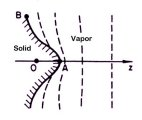
\includegraphics{branching-start.jpg}
		\caption{Rozgałęzianie}
	\end{figure}
\end{frame}


\begin{frame}
	\frametitle{Rozgałęzianie}
	\begin{block}{Dendryty}
		Kiedy niestabilność rozgałęziająca aplikuje się nieustannie do rosnącego kryształu, powstaje drzewiasta struktura zwana dendrytem.	
	\end{block}
\end{frame}

\begin{frame}
	\frametitle{Bibliografia}
	\begin{block}{Bibliografia}
		\begin{itemize}
	 		\item SnowCrystals - http://www.its.caltech.edu/~atomic/snowcrystals
		\end{itemize}
	\end{block}
\end{frame}

\section{Plan rozwoju}

\subsection{Wersja I}

\begin{frame}
	\frametitle{Wersja I}
	\begin{block}{Rezultat}
		\begin{itemize}
	 		\item Pojedyńcze jądro kondensacji
			\item Zależność od chęci agenta do przyłączenia i jego prędkości dyfuzji.
			\item Dwie naprzemienne fazy cyklu życia agenta: dyfuzja i przyłączanie 
			\item Dwuwymiarowość
		\end{itemize}
	\end{block}
\end{frame}


\subsection{Wersja II}

\begin{frame}
	\frametitle{Wersja II}
	\begin{block}{Rezultat}
		\begin{itemize}
	 		\item Pojedyńcze jądro kondensacji
			\item Zależność od temperatury i wilgotności.
			\item Pięć naprzemiennych faz cyklu życia agenta: dyfuzja, zamarzanie, przyłączanie, topnienie, zakłócenie 
			\item Trójwymiarowość zrealizowana poprzez cieniowanie.
		\end{itemize}
	\end{block}
\end{frame}



\subsection{Wersja III}

\begin{frame}
	\frametitle{Wersja III}
	\begin{block}{Rezultat}
		\begin{itemize}
	 		\item Wiele jąder kondensacji
			\item Zależność od temperatury i wilgotności.
			\item Pięć naprzemiennych faz cyklu życia agenta: dyfuzja, zamarzanie, przyłączanie, topnienie, zakłócenie 
			\item Trójwymiarowość.
		\end{itemize}
	\end{block}
\end{frame}


\end{document}


